\documentclass[a4paper]{article}
\usepackage[utf8]{inputenc}
\usepackage{amsmath,amsthm,amsfonts,amssymb,amscd}
\usepackage{multirow,booktabs}
\usepackage{tabularx}
\usepackage{longtable}
\usepackage{listings}
\usepackage{color}
\lstset{
  basicstyle=\footnotesize,
  breaklines=true,
  frame=single,
  keepspaces=true,
  language=Python,
  numbers=left,
  numbersep=5pt,
  numberstyle=\tiny\color{gray}
}
\usepackage{hyperref}
\hypersetup{
    colorlinks=true,
    linkcolor=blue,
    citecolor=black,
    filecolor=black,
    urlcolor=purple,
    linktoc=page
}
\usepackage{float}
\usepackage{subcaption}
\usepackage[table]{xcolor}
\usepackage{fullpage}
\usepackage{lastpage}
\usepackage{ulem}
\usepackage{enumitem}
\usepackage{fancyhdr}
\usepackage{mathrsfs}
\usepackage{wrapfig}
\usepackage{setspace}
\usepackage{calc}
\usepackage{multicol}
\usepackage{cancel}
\usepackage[retainorgcmds]{IEEEtrantools}
\usepackage[margin=3cm]{geometry}
\usepackage{amsmath}
\newlength{\tabcont}
\setlength{\parindent}{0.0in}
\setlength{\parskip}{0.05in}
\usepackage{empheq}
\usepackage{framed}
\usepackage[most]{tcolorbox}
\usepackage{xcolor}
\usepackage{graphicx}
\usepackage{caption}
\usepackage{pdflscape}
\graphicspath{{./chapters/images}}
\colorlet{shadecolor}{orange!15}
\parindent 0in
\parskip 12pt
\geometry{margin=1in, headsep=0.25in}
\theoremstyle{definition}
\newtheorem{defn}{Definition}
\newtheorem{reg}{Rule}
\newtheorem{exer}{Exercise}
% \newtheorem{note}{Note}
\newenvironment{note}
  {\par\textbf{Note:}\quad}
  {\par}

\begin{document}
\begin{center}
    {\LARGE \bf     Weekly reports for IARCS Internship}\\[9pt]
    {\large Wong Chu Feng}\\[8pt]
    {Jan - May 2024}
\end{center}
\tableofcontents
\clearpage

\section*{Week 1: Research on STRIDE and Mitre ATT\&CK}
\addcontentsline{toc}{section}{Week 1: Research on STRIDE and Mitre ATT\&CK}
Pointers:
\begin{itemize}
    \item Read up on STRIDE framework, MITRE ATT\&CK and OpenAI's API.
    \item Briefing on internship, phase 1 and 2.\\
    \includegraphics*[scale=1.1]{work.png}
    \item Studied code from current stride (supervised) \href{https://github.com/sebyakuya/stride-classifier/tree/master}{model classifier}.
    \item Understood the supervised model's code. Looking at the $raw\_capec\_data.xlsx$ to try clustering methods to create an unsupervised model. The trained supervised model might be useful in feature extraction to train the unsupervised model. What features exactly? Or in transfer learning? Still not too sure.
    \item Digressing a bit, started researching for similar papers on mapping ATT\&CK to STRIDE.
    \item Discovered \href{https://github.com/center-for-threat-informed-defense/tram}{TRAM LLM} $\rightarrow$ \textit{Possible to use with the questionaire from GovTech as an input.}
        \begin{itemize}
            \item identifies keywords, capable of contextual understanding
            \item predicts the presence of TTPs (Tactics, Techniques, Procedures) in the text
            \item then \href{https://github.com/center-for-threat-informed-defense/tram/wiki/Using-TRAM#machine-learning}{finds} the corresponding ATT\&CK technique(s).\\
            \includegraphics*[scale=0.4]{tramllm.png}
        \end{itemize}
    \item \href{https://arxiv.org/pdf/2206.10272.pdf}{Identification of Attack Paths Using Kill Chain and Attack Graphs} $\rightarrow$ \textit{Needs a separate function to create this graph. Seemingly not helpful.}\\
    \includegraphics*[scale=0.28]{poss_questionaire.png}
    \includegraphics*[scale=0.32]{poss_questionairediag.png}
    \item Thinking of either a standalone unsupervised model or a \href{https://journalofbigdata.springeropen.com/articles/10.1186/s40537-022-00636-w}{hybrid} one.
    \item Summary: Make use of the current supervised model that maps Mitre Att\&cks using keywords to STRIDE. Then we can spatially obtain the clusters of data each corresponding to a category in STRIDE. We can use this as the baseline to train the unsupervised model. Each similarity of \textit{category from GovTech} will be weighted against STRIDE, thereby allowing the mapping of STRIDE to \textit{the GovTech framework}.
    \item Consolidate ideas:
        \begin{itemize}
            \item Use unsupervised model.
            \item Use hybrid model. Use the current supervised model to extract features (if any) and pass it to the unsupervised model to train for the $GovTech$ framework.
            \item Find the similarities between STRIDE and the \textit{GovTech framework}, give each category some keywords and use DL to find its weights. Then use the weights to train the unsupervised model.
        \end{itemize}
    \item Attempt to change the current supervised model to an unsupervised one.
\end{itemize}
\clearpage
\section*{Week 2: Building the model}
\addcontentsline{toc}{section}{Week 2: Building the model}

Attempted at using \textit{Tokenizer} for feature extraction. Yields 0.469 accuracy. Should be due to the corpus being too small for the model to properly learn the context of the words.
\begin{lstlisting}[frame=single]
tokenizer = Tokenizer(oov_token='<OOV>')
tokenizer.fit_on_texts(df_train['NameDesc'])
X_train = tokenizer.texts_to_sequences(df_train['NameDesc'])
X_test = tokenizer.texts_to_sequences(df_test['NameDesc'])
X_val = tokenizer.texts_to_sequences(df_dev['NameDesc'])

x = [X_train, X_test, X_val]
max_length = 0
for _ in x:
    max_l = max([len(seq) for seq in _])
    max_length = max(max_length, max_l)

X_train_padded = pad_sequences(X_train, maxlen=max_length, padding='post')
X_test_padded = pad_sequences(X_test, maxlen=max_length, padding='post')
X_val_padded = pad_sequences(X_val, maxlen=max_length, padding='post')

y_train = df_train['STRIDE'].values
y_test = df_test['STRIDE'].values
y_val = df_dev['STRIDE'].values
\end{lstlisting}

Second attempt using \textit{TfidfVectorizer} for feature extraction. This model performs better because TfidfVectorizer works better with a small corpus as it takes into account the frequency of the words appearing which might indicate keywords of a STRIDE category.
\begin{lstlisting}[frame=single]
tfidf_vectorizer = TfidfVectorizer()

X_train_tfidf = tfidf_vectorizer.fit_transform(df_train['NameDesc']).toarray()
X_test_tfidf = tfidf_vectorizer.transform(df_test['NameDesc']).toarray()
X_val_tfidf = tfidf_vectorizer.transform(df_dev['NameDesc']).toarray()

y_train = df_train['STRIDE'].values
y_test = df_test['STRIDE'].values
y_val = df_dev['STRIDE'].values
\end{lstlisting}

Then I perform hyperparameter tuning on the model.:
\begin{lstlisting}[frame=single]
dropout_rates = [0.2, 0.3, 0.4, 0.5]
activations_list = ['relu', 'leaky_relu', 'elu', 'tanh']
num_neurons = [32, 64, 128, 256]
opt_lr = [1e-2, 1e-3, 1e-4]
L2_lr = [1e-2, 1e-3, 1e-4]
best_params = None
best_val_acc = 0

hyperparam_combi = itertools.product(dropout_rates, num_neurons, activations_list, opt_lr, L2_lr)

for dr, nn, al, olr, l2lr in hyperparam_combi:
    modelTest = tf.keras.Sequential([
    tf.keras.layers.Input(shape=(vocab_size,)),
    tf.keras.layers.Dense(nn*2, activation=al),
    tf.keras.layers.Dropout(dr),
    tf.keras.layers.BatchNormalization(),
    tf.keras.layers.Dense(nn, activation=al),
    tf.keras.layers.Dropout(dr),
    tf.keras.layers.BatchNormalization(),
    tf.keras.layers.Dense(nn//2, activation=al),
    tf.keras.layers.Dense(num_classes, kernel_regularizer=tf.keras.regularizers.L2(l2=1e-2), activation='softmax')
    ])

    optimizer = tf.keras.optimizers.legacy.Adam(olr)
    modelTest.compile(optimizer=optimizer, loss="sparse_categorical_crossentropy", metrics=['accuracy'])
    
    early_stop = EarlyStopping(
        monitor="val_loss",
        patience=5,
        verbose=0,
        restore_best_weights=True
    )
    histTest = modelTest.fit(
        X_train_tfidf, y_train,
        batch_size=16,
        epochs=num_epochs,
        validation_data=(X_val_tfidf, y_val),
        verbose=0,
        callbacks=[early_stop,]
    )

    val_acc = max(histTest.history['val_accuracy'])
    # print(f"Dropout: {dr}, Activation: {al}, Hidden Units: {nn}, L2 Reg: {l2lr}, LR: {olr}, Best Val Acc: {val_acc}\n===========================")
    if val_acc > best_val_acc:
        best_val_acc = val_acc
        best_params = (dr, nn, al, olr, l2lr)
\end{lstlisting}

Final Best Hyperparameters:\\
Dropout: \textit{0.2},\\
Activation: \textit{elu},\\
Hidden Units: \textit{32},\\
L2 Reg: \textit{0.001},\\
LR: \textit{0.0001},\\
Best Val Acc: 0.\textit{918367326259613}\\

Final model used:
\begin{lstlisting}[frame=single]
hidden_units = 32
num_classes = 6
batch_size = 16
num_epochs = 50
classes = [0,1,2,3,4,5]
vocab_size = X_train_tfidf.shape[1]
optimizer = tf.keras.optimizers.legacy.Adam(1e-4)

model3 = tf.keras.Sequential([
    tf.keras.layers.Input(shape=(vocab_size,)),
    tf.keras.layers.Dense(hidden_units*2, activation='elu'),
    tf.keras.layers.Dropout(.2),
    tf.keras.layers.BatchNormalization(),
    tf.keras.layers.Dense(hidden_units, activation='elu'),
    tf.keras.layers.Dropout(.2),
    tf.keras.layers.BatchNormalization(),
    tf.keras.layers.Dense(hidden_units//2, activation='elu'),
    tf.keras.layers.Dense(num_classes, kernel_regularizer=tf.keras.regularizers.L2(l2=1e-3), activation='softmax')
])

model3.compile(optimizer=optimizer, loss="sparse_categorical_crossentropy", metrics=['accuracy'])
model3.summary()
# plot_model(model3, show_shapes=True, show_layer_names=True)
\end{lstlisting}
\clearpage
Results:
Plotted a confusion matrix to evaluate the model. It yields an accuracy of 0.857 where the diagonal entries are the true labels predicted.
\begin{figure}[!h]
    \includegraphics*[scale=0.528]{cmatrix_1.png}
\end{figure}

Summary:
\vspace{-\baselineskip}
\begin{itemize}
    \item Try fuzzy clustering on the dataset since GMM and DBSCAN proves to be not too helpful.
    \item Attempt pulling out more specific keywords and predict the STRIDE category
    \item Examine using one model for each of STRIDE category
\end{itemize}
\clearpage
\section*{Week 3: Finding better models}
\addcontentsline{toc}{section}{Week 3: Finding better models}

\textbf{Note: }I discovered an error in the code for the previous model shown in week 2 where the promising results were ultimately spurious.

This is a more aggressive text preprocessing on the corpus. I first conduct a preliminary analysis of the word frequencies and trivially remove unimportant words.
\begin{lstlisting}[frame=single]
def basic_processing(df):
    words_to_remove = ["e.g.", "code", "may", "attack", "system", "adversary", "Adversaries"]
    for word in words_to_remove:
        df['NameDesc'] = df['NameDesc'].apply(lambda x: x.replace(word, ''))
    for word in words_to_remove:
        df['NameDesc'] = df['NameDesc'].apply(lambda x: re.sub(r'\b' + re.escape(word) + r'\b', '', x))

    # df['NameDesc'] = df['NameDesc'].str.replace(r"\b(" + "|".join(words_to_remove) + r")\b", "", regex=True)
    df['NameDesc'] = df['NameDesc'].str.replace("<br><br>", "", regex=True)
    df['NameDesc'] = df['NameDesc'].str.replace("\(Citation:.*?\)", "", regex=True)
    df['NameDesc'] = df['NameDesc'].str.replace("http\S+", "", regex=True)
    df['NameDesc'] = df['NameDesc'].str.replace("  +", " ", regex=True)
    df['NameDesc'] = df['NameDesc'].str.replace("[^A-Za-z]", " ", regex=True)
    return df

def rm_stopwords(df):
    stop_words = set(stopwords.words('english'))
    df['NameDesc'] = df['NameDesc'].apply(lambda x: [word for word in x if word not in stop_words])
    print(f"Removed stopwords:\n {df.head(3).NameDesc}\n")
    return df

def lemmatize(df):
    lemmatizer = WordNetLemmatizer()
    def lemmatize_tokens(tokens):
        def get_wordnet_pos(word):
            tag = nltk.pos_tag([word])[0][1][0].upper()
            tag_dict = {"J": wordnet.ADJ,
                        "N": wordnet.NOUN,
                        "V": wordnet.VERB,
                        "R": wordnet.ADV}
            return tag_dict.get(tag, wordnet.NOUN)
        lemmas = [lemmatizer.lemmatize(token, get_wordnet_pos(token)) for token in tokens]
        return lemmas
    df['NameDesc'] = df['NameDesc'].apply(lambda x: lemmatize_tokens(x))
    print(f"Lemmatized words:\n {df.head(3).NameDesc}")
    return df

def text_preprocessing(df):
    basic_processing(df)
    df['NameDesc'] = df['NameDesc'].apply(lambda x: word_tokenize(x))
    rm_stopwords(df)
    lemmatize(df)
    print("=========================================")
    return df
\end{lstlisting}

\begin{table}[h]
    \caption{Extracting keywords}
    \label{crouch}
    \begin{tabularx}{\textwidth}{p{0.1\textwidth}XX}
        \toprule
        \textbf{Dataset} & \textbf{Original text} & \textbf{Stemmed \& Lemmatized text} \\
        \midrule
        df\_train[0] &
        Exfiltration to Cloud Storage Adversaries may exfiltrate data to a cloud storage service rather than over their primary command and control channel. Cloud storage services allow for the storage, edit, and retrieval of data from a remote cloud storage server over the Internet. Examples of cloud storage services include Dropbox and Google Docs. Exfiltration to these cloud storage services can provide a significant amount of cover to the adversary if hosts within the network are already communicating with the service. Analyze network data for uncommon data flows (e.g., a client sending significantly more data than it receives from a server) to known cloud storage services. Processes utilizing the network that do not normally have network communication or have never been seen before are suspicious. User behavior monitoring may help to detect abnormal patterns of activity.
        &
        [Exfiltration, Cloud, Storage, exfiltrate, data, cloud, storage, service, rather, primary, command, control, channel, Cloud, storage, service, allow, storage, edit, retrieval, data, remote, cloud, storage, server, Internet, Examples, cloud, storage, service, include, Dropbox, Google, Docs, Exfiltration, cloud, storage, service, provide, significant, amount, cover, host, within, network, already, communicate, service, Analyze, network, data, uncommon, data, flow, client, send, significantly, data, receives, server, know, cloud, storage, service, Processes, utilize, network, normally, network, communication, never, see, suspicious, User, behavior, monitoring, help, detect, abnormal, pattern, activity] \\
        \midrule
        df\_train[2] &
        Runtime Data Manipulation Adversaries may modify systems in order to manipulate the data as it is accessed and displayed to an end user, thus threatening the integrity of the data.(Citation: FireEye APT38 Oct 2018)(Citation: DOJ Lazarus Sony 2018) By manipulating runtime data, adversaries may attempt to affect a business process, organizational understanding, and decision making.<br><br>Adversaries may alter application binaries used to display data in order to cause runtime manipulations. Adversaries may also conduct [Change Default File Association]\nolinkurl{(https://attack.mitre.org/techniques/T1546/001)} and [Masquerading]\nolinkurl{(https://attack.mitre.org/techniques/T1036)} to cause a similar effect. The type of modification and the impact it will have depends on the target application and process as well as the goals and objectives of the adversary. For complex systems, an adversary would likely need special expertise and possibly access to specialized software related to the system that would typically be gained through a prolonged information gathering campaign in order to have the desired impact.\verb|<br><br>|Inspect important application binary file hashes, locations, and modifications for suspicious/unexpected values.
        &
        [Runtime, Data, Manipulation, modify, order, manipulate, data, access, displayed, end, user, thus, threaten, integrity, data, By, manipulate, runtime, data, adversary, attempt, affect, business, process, organizational, understand, decision, make, alter, application, binary, use, display, data, order, cause, runtime, manipulation, also, conduct, Change, Default, File, Association, Masquerading, cause, similar, effect, The, type, modification, impact, depends, target, application, process, well, goal, objective, For, complex, would, likely, need, special, expertise, possibly, access, specialized, software, related, would, typically, gain, prolong, information, gathering, campaign, order, desire, impact, Inspect, important, application, binary, file, hash, location, modification, suspicious, unexpected, value] \\
        \bottomrule
    \end{tabularx}
\end{table}
\clearpage
Visualising the word frequencies in the corpus:\\
Using TfidfVectorizer and after hyperparameter tuning, the model to use is as follows.
\begin{lstlisting}[frame=single]
hidden_units = 32
batch_size = 16
num_epochs = 50
num_classes = 6
classes = [0,1,2,3,4,5]
vocab_size = X_train_tfidf.shape[1]
optimizer = tf.keras.optimizers.legacy.Adam(1e-4)

model4 = tf.keras.Sequential([
    tf.keras.layers.Input(shape=(vocab_size,)),
    tf.keras.layers.Dense(hidden_units*2, activation='elu'),
    tf.keras.layers.Dropout(.5),
    tf.keras.layers.BatchNormalization(),
    tf.keras.layers.Dense(hidden_units, activation='elu'),
    tf.keras.layers.Dropout(.5),
    tf.keras.layers.BatchNormalization(),
    tf.keras.layers.Dense(hidden_units//2, activation='elu'),
    tf.keras.layers.Dense(num_classes, kernel_regularizer=tf.keras.regularizers.L2(l2=1e-2), activation='softmax')
])
r
model4.compile(optimizer=optimizer, loss="sparse_categorical_crossentropy", metrics=['accuracy'])
model4.summary()
# plot_model(model4, show_shapes=True, show_layer_names=True)
\end{lstlisting}

This model predicts with accuracy of 0.79.\\
\includegraphics*[scale=0.528]{cmatrix_model4.png}
\clearpage
\textbf{Attempt on Fuzzy Clustering}\\
\begin{table}[h]
    \caption{Extracting keywords}
    \label{crouch}
    \begin{tabularx}{\textwidth}{p{0.1\textwidth}X}
        \toprule
        \textbf{Cluster} & \textbf{Unique STRIDE values} \\
        \midrule
        0 &
        ['000001' '010000' '000100' '000010' '110000' '010001' '100000' '101000' '100100' '011000'] \\
        \midrule
        1 &
        ['000010' '010000' '000001' '000100' '100000' '010010' '011000' '100001' '100100' '101000'] \\
        \midrule
        2 &
        ['000001' '010000' '000100'] \\
        \midrule
        3 &
        ['011000'] \\
        4 &
        ['000001' '010000' '010100' '000100' '100000'] \\
        5 &
        ['010001' '000001' '010000' '011000' '000010' '000100' '100100' '100000'] \\
        \bottomrule
    \end{tabularx}
\end{table}

Visualising the clusters:\\
\includegraphics*[scale=0.75]{fuzzyclustering.png}

\vspace*{10pt}
Moving forward, there are several improvements to be made.
\begin{itemize}
    \item Instead of selecting keywords from the corpus, it can be constructed by hand using the definition of each categories of STRIDE, and subsequently of RAPIDS.
    \item Filtering of keywords can include more manual methods to further reduce the keyword corpus.
    \item Visualise and examine the frequencies for some keywords and manually remove some, then we will be left with lesser keywords that the model will be used to train on, potentially increasing the accuracy of classification.
\end{itemize}
\clearpage
\section*{Week 4: Refining the corpus and model}
\addcontentsline{toc}{section}{Week 4: Refining the corpus and model}

Improvement 1: Removed duplicate words\\
\begin{table}[h]
    \caption{Extracting keywords v2.0}
    \label{crouch}
    \begin{tabularx}{\textwidth}{p{0.1\textwidth}XX}
        \toprule
        \textbf{Dataset} & \textbf{Original text} & \textbf{Processed text} \\
        \midrule
        df\_train[0] &
        Business Relationships Adversaries may gather information about the victim's business relationships that can be used during targeting. Information about an organization's business relationships may include a variety of details, including second or third-party organizations/domains (ex: managed service providers, contractors, etc.) that have connected (and potentially elevated) network access. This information may also reveal supply chains and shipment paths for the victim's hardware and software resources.\verb|<br><br>|Adversaries may gather this information in various ways, such as direct elicitation via [Phishing for Information]\nolinkurl{(https://attack.mitre.org/techniques/T1598)}. Information about business relationships may also be exposed to adversaries via online or other accessible data sets (ex: [Social Media]\nolinkurl{(https://attack.mitre.org/techniques/T1593/001)} or [Search Victim-Owned Websites]\nolinkurl{(https://attack.mitre.org/techniques/T1594)}).(Citation: ThreatPost Broadvoice Leak) Gathering this information may reveal opportunities for other forms of reconnaissance (ex: [Phishing for Information]\nolinkurl{(https://attack.mitre.org/techniques/T1598)} or [Search Open Websites/Domains]\nolinkurl{(https://attack.mitre.org/techniques/T1593)}), establishing operational resources (ex: [Establish Accounts]\nolinkurl{(https://attack.mitre.org/techniques/T1585)} or [Compromise Accounts]\nolinkurl{(https://attack.mitre.org/techniques/T1586)}), and/or initial access (ex: [Supply Chain Compromise]\nolinkurl{(https://attack.mitre.org/techniques/T1195)}, [Drive-by Compromise]\nolinkurl{(https://attack.mitre.org/techniques/T1189)}, or [Trusted Relationship]\nolinkurl{(https://attack.mitre.org/techniques/T1199)}).\verb|<br><br>|Much of this activity may have a very high occurrence and associated false positive rate, as well as potentially taking place outside the visibility of the target organization, making detection difficult for defenders.\verb|<br><br>|Detection efforts may be focused on related stages of the adversary lifecycle, such as during Initial Access.
        &
        ['websites', 'associate', 'contractor', 'supply', 'path', 'online', 'variety', 'operational', 'this', 'phishing', 'gathering', 'via', 'search', 'use', 'adversary', 'open', 'take', 'initial', 'drive', 'victim', 'include', 'etc', 'manage', 'potentially', 'trusted', 'access', 'connect', 'target', 'resource', 'elicitation', 'hardware', 'organization', 'direct', 'place', 'rate', 'elevate', 'network', 'service', 'well', 'domains', 'second', 'activity', 'gather', 'way', 'establish', 'stage', 'provider', 'compromise', 'data', 'defender', 'relationship', 'false', 'chain', 'reconnaissance', 'accounts', 'media', 'social', 'relationships', 'outside', 'information', 'effort', 'domain', 'detail', 'related', 'business', 'software', 'various', 'also', 'opportunity', 'lifecycle', 'ex', 'set', 'owned', 'positive', 'detection', 'third', 'accessible', 'party', 'high', 'difficult', 'occurrence', 'make', 'shipment', 'visibility', 'focus', 'reveal', 'expose', 'form'] \\
        \midrule
        df\_train[2] &
        Symmetric Cryptography Adversaries may employ a known symmetric encryption algorithm to conceal command and control traffic rather than relying on any inherent protections provided by a communication protocol. Symmetric encryption algorithms use the same key for plaintext encryption and ciphertext decryption. Common symmetric encryption algorithms include AES, DES, 3DES, Blowfish, and RC4.\verb|<br><br>|With symmetric encryption, it may be possible to obtain the algorithm and key from samples and use them to decode network traffic to detect malware communications signatures.\verb|<br><br>|In general, analyze network data for uncommon data flows (e.g., a client sending significantly more data than it receives from a server). Processes utilizing the network that do not normally have network communication or have never been seen before are suspicious. Analyze packet contents to detect communications that do not follow the expected protocol behavior for the port that is being used.(Citation: University of Birmingham C2)
        &
        ['content', 'sample', 'packet', 'know', 'obtain', 'data', 'flow', 'provide', 'with', 'uncommon', 'control', 'utilize', 'traffic', 'port', 'key', 'general', 'detect', 'de', 'algorithm', 'see', 'send', 'rc', 'follow', 'decryption', 'suspicious', 'employ', 'protection', 'processes', 'plaintext', 'cryptography', 'malware', 'ciphertext', 'inherent', 'analyze', 'never', 'conceal', 'behavior', 'use', 'in', 'signature', 'symmetric', 'command', 'common', 'possible', 'network', 'include', 'aes', 'encryption', 'protocol', 'server', 'rather', 'rely', 'blowfish', 'receives', 'des', 'expect', 'communication', 'significantly', 'normally', 'client'] \\
        \bottomrule
    \end{tabularx}
\end{table}

\clearpage
\textbf{Figuring out keywords using Microsoft's definition of STRIDE}\\\\

\textbf{S:} Involves illegally accessing and then using another user's authentication information, such as username and password \\\\
\textbf{T:} Involves the malicious modification of data. Examples include unauthorized changes made to persistent data, such as that held in a database, and the alteration of data as it flows between two computers over an open network, such as the Internet \\\\
\textbf{R:} Associated with users who deny performing an action without other parties having any way to prove otherwise—for example, a user performs an illegal operation in a system that lacks the ability to trace the prohibited operations. Non-Repudiation refers to the ability of a system to counter repudiation threats. For example, a user who purchases an item might have to sign for the item upon receipt. The vendor can then use the signed receipt as evidence that the user did receive the package \\\\
\textbf{I:} Involves the exposure of information to individuals who are not supposed to have access to it—for example, the ability of users to read a file that they were not granted access to, or the ability of an intruder to read data in transit between two computers \\\\
\textbf{D:} Denial of service (DoS) attacks deny service to valid users—for example, by making a Web server temporarily unavailable or unusable. You must protect against certain types of DoS threats simply to improve system availability and reliability \\\\
\textbf{E:} An unprivileged user gains privileged access and thereby has sufficient access to compromise or destroy the entire system. Elevation of privilege threats include those situations in which an attacker has effectively penetrated all system defenses and become part of the trusted system itself, a dangerous situation indeed \\\\

\textbf{Create keywords from the definitions}\\\\
\textbf{S:} ['authenticate', 'username', 'password', 'access'] \\\\
\textbf{T:} ['modify', 'persistent', 'database', 'alter', 'open', 'network', 'internet'] \\\\ % persistent data as in the data that is not meant to be modified and infrequently accessed
\textbf{R:} ['deny', 'action', 'prove', 'non-repudiation', 'item', 'sign', 'receipt', 'receive', 'evidence', 'package', 'untrace',] \\\\
\textbf{I:} ['exposure', 'individual', 'access', 'file', 'granted', 'intruder', 'transit'] \\\\
\textbf{D:} ['denial', 'service', 'dos', 'web', 'server', 'unavailable', 'unusable', 'system', 'available', 'reliable'] \\\\
\textbf{E:} ['unprivileged', 'privileged', 'access', 'compromise', 'entire', 'system', 'elevation', 'penetrate', 'defenses', 'untrusted', 'trusted'] \\\\

\textbf{Keywords obtained from manually filtering the corpus}\\\\
\textbf{S\_keep:} ['information', 'detection', 'take',  'include', 'malicious', 'control', 'network', 'search', 'name', 'access', 'infrastructure', 'traffic', 'data', 'suspicious', 'trust', 'reconnaissance', 'email', 'phishing', 'resource', 'initial', 'visibility', 'monitor', 'server', 'form', 'open', 'potentially', 'websites', 'address', 'process', 'detect', 'credential', 'file', 'certificate', 'internet', 'install', 'key', 'online', 'link', 'source'] \\\\
\textbf{T\_keep:} ['malicious', 'file', 'activity', 'process', 'execute', 'access', 'information', 'control', 'software', 'modify', 'network', 'data', 'abuse', 'exe', 'manipulate', 'bypass', 'malware', 'functionality', 'integrity', 'dll', 'anomaly', 'install'] \\\\
\textbf{R\_keep:} ['user', 'application', 'api', 'activity', 'audit', 'source', 'system', 'native', 'hide', 'error', 'intrusion', 'function', 'record', 'clear', 'gcp', 'permission', 'analysis', 'collection', 'updatesink', 'indicate', 'detection', 'data', 'collect', 'environment', 'call', 'limit', 'cloudtrail', 'loss', 'conduct', 'prior', 'delete', 'cloud', 'configservicev', 'cloudwatch', 'diagnostic', 'capability', 'sufficient', 'insight', 'avoid'] \\\\
\textbf{I\_keep:} ['data', 'network', 'activity', 'access', 'behavior', 'environment', 'process', 'detection', 'remote', 'base', 'target', 'tool', 'file', 'api', 'traffic', 'acquire', 'application', 'host', 'infrastructure', 'device'] \\\\
\textbf{D\_keep:} ['service', 'target', 'tool', 'command', 'cause', 'server', 'network', 'outside', 'denial', 'dos', 'availability', 'high', 'destruction', 'infrastructure'] \\\\
\textbf{E\_keep:} ['process', 'access', 'file', 'execute', 'activity', 'execution', 'network', 'behavior', 'create', 'control', 'log', 'privilege', 'application', 'service', 'within', 'event', 'account', 'modify', 'run', 'abuse', 'monitoring', 'environment', 'binary', 'credential', 'enable', 'api', 'exe', 'function', 'payload', 'target', 'method', 'services', 'launch', 'root', 'os', 'many''accounts'] \\\\

Now, merge both lists together by group to get for example \textit{S\_final}. \\

Summary: Next week, to compare the semantic similarity of keywords to choose the final set of keywords to use for training the model. If it does not work, I will look into the Large Language Model Meta AI \(LLaMA\) language model.
\clearpage
\section*{Week 5: Solution for selecting final set of keywords}
\addcontentsline{toc}{section}{Week 5: Solution for selecting final set of keywords}

Continuing from last week: With respect to each STRIDE cateogry, when referencing the list keywords we just obtained, eg. \textit{S\_final}, and the initial list of keywords we obtained, there exists an underlying problem where we are unsure of which words should be deleted or kept for training the model.\\
The solution I implemented using \textit{word2vec} to compare both lists and compare the similarities between words and set a minimum cosine value threshold. Any words with similarities below the threshold are deemed 'not similar enough' and will be dropped. \\
Through experimentation, the threshold value selected is 0.28. An example can be found in \hyperref[subsec:appendix2]{Appendix 2}\\

\begin{lstlisting}[frame=single]
def merge_lists(l1, min_cosine_value, w2v, ref_list):
final_list = []

for word in l1:
    if word in w2v:
        similarities = []
        for ref_word in ref_list:
            if ref_word in w2v:
                sim = w2v.similarity(word, ref_word)
                similarities.append(sim)
        if any(sim >= min_cosine_value for sim in similarities):
            final_list.append(word)
if 'use' in final_list: final_list.remove('use')
elif 'also' in final_list: final_list.remove('also')
return final_list
\end{lstlisting}

\begin{table}[h]
    \caption{Comparing keywords (arbitary example)}
    \label{crouch}
    \begin{tabularx}{\textwidth}{p{0.3\textwidth}XX}
        \toprule
        \textbf{Original set} & \textbf{Manually filtered set} & \textbf{Resultant set + words removed by semantic analysis} \\
        \midrule
        domain, activity, high, direct, include, path, relationship, network, gather, visibility, software, potentially, difficult, make, trusted, supply, gathering, manage, access, form, via, compromise, place, accounts, business, information, focus, elicitation, lifecycle, drive, defender, second, effort, set, provider, take, victim, social, owned, outside, phishing, operational, positive, reconnaissance, stage, domains, party, associate, way, false, variety, chain, well, connect, service, hardware, opportunity, various, online, organization, detection, search, accessible, this, media, target, use, elevate, detail, initial, data, adversary, related, reveal, occurrence, establish, third, etc, expose, relationships, resource, shipment, contractor, ex, open, rate, websites, also
        &
        authenticate, username, password, access, information, detection, take, include, malicious, control, network, search, name, access, infrastructure, traffic, data, suspicious, trust, reconnaissance, email, phishing, resource, initial, visibility, monitor, server, form, open, potentially, websites, address, process, detect, credential, file, certificate, internet, install, key, online, link, source
        &
        domain, include, relationship, network, gather, visibility, software, potentially, make, trusted, manage, access, form, via, information, lifecycle, provider, take, phishing, operational, reconnaissance, domains, connect, service, hardware, online, organization, detection, search, accessible, media, use, initial, data, reveal, establish, expose, relationships, resource, open, websites, \sout{source, file, malicious, certificate, monitor, authenticate, suspicious, email, install, server, link, detect, control, trust, address, credential, internet, process, password, traffic, key, username, name, infrastructure} \\
        \bottomrule
    \end{tabularx}
\end{table}
\clearpage

A word cloud for each STRIDE category is generated to visualise the keywords.
\begin{figure}[h]
    \centering
    \begin{subfigure}{0.45\textwidth}
        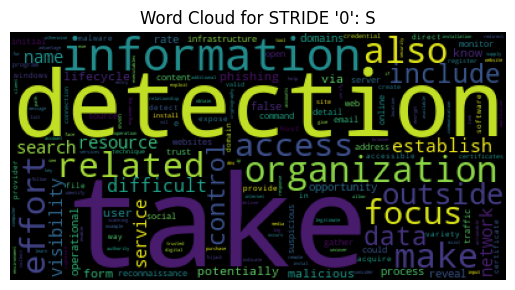
\includegraphics[width=\linewidth]{wordcloud/wc_0S.png}
    \end{subfigure}
    \hfill
    \begin{subfigure}{0.45\textwidth}
        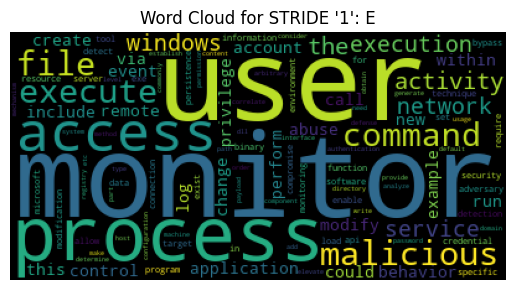
\includegraphics[width=\linewidth]{wordcloud/wc_1E.png}
    \end{subfigure}
    
    \medskip
    
    \begin{subfigure}{0.45\textwidth}
        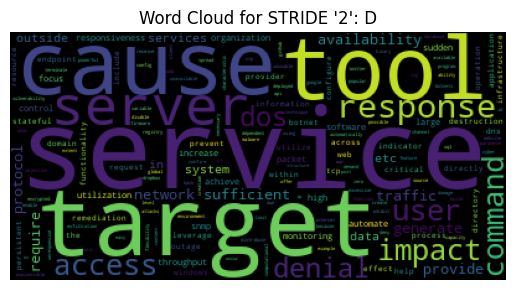
\includegraphics[width=\linewidth]{wordcloud/wc_2D.png}
    \end{subfigure}
    \hfill
    \begin{subfigure}{0.45\textwidth}
        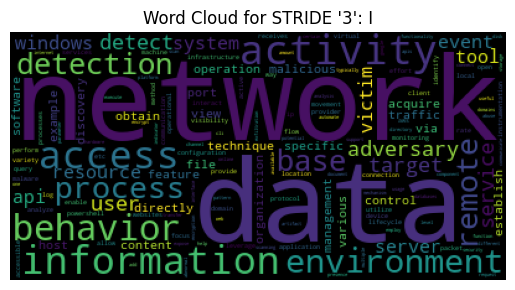
\includegraphics[width=\linewidth]{wordcloud/wc_3I.png}
    \end{subfigure}
    
    \medskip
    
    \begin{subfigure}{0.45\textwidth}
        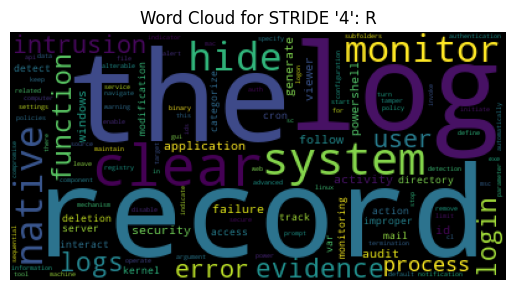
\includegraphics[width=\linewidth]{wordcloud/wc_4R.png}
    \end{subfigure}
    \hfill
    \begin{subfigure}{0.45\textwidth}
        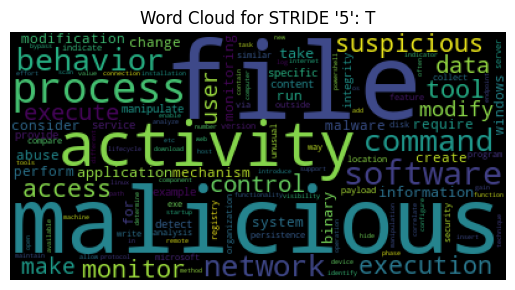
\includegraphics[width=\linewidth]{wordcloud/wc_5T.png}
    \end{subfigure}
    \label{fig:grid}
\end{figure}

Moving on, using the right most column of Table 5, I tokenize them and pass it into a multi-layer perceptron model where it is fine-tuned by hyperparamter testing (\hyperref[subsec:appendix3]{Appendix 3}). \\
\begin{lstlisting}[frame=single]
hidden_units = 128
batch_size = 16
num_epochs = 50
num_classes = 6
classes = [0,1,2,3,4,5]
vocab_size = X_train_tfidf.shape[1]
optimizer = tf.keras.optimizers.legacy.Adam(1e-4)

model5 = tf.keras.Sequential([
    tf.keras.layers.Input(shape=(vocab_size,)),
    tf.keras.layers.Dense(hidden_units*2, activation='leaky_relu'),
    tf.keras.layers.Dropout(.2),
    tf.keras.layers.BatchNormalization(),
    tf.keras.layers.Dense(hidden_units, activation='leaky_relu'),
    tf.keras.layers.Dropout(.2),
    tf.keras.layers.BatchNormalization(),
    tf.keras.layers.Dense(hidden_units//2, activation='leaky_relu'),
    tf.keras.layers.Dense(num_classes, kernel_regularizer=tf.keras.regularizers.L2(l2=1e-3), activation='softmax')
])

model5.compile(optimizer=optimizer, loss="sparse_categorical_crossentropy", metrics=['accuracy'])
model5.summary()
\end{lstlisting}

The results of this model is as follows:\\
\includegraphics*[scale=0.528]{cmatrix_model5.png}

This model seems to perform terribly on 'T' and 'E' categories.

Some improvements to be done:
\begin{itemize}[topsep=0pt]
    \item Create a separate model to classify 'T' and 'E' as they yield low accuracies. Then try to combine these models with \textit{model5}
    \item Evaluate the usefulness of \textit{LLaMA} model
\end{itemize}
\clearpage
\section*{Week 6: Experimenting with Llama 2 \& different training technqiues}
\addcontentsline{toc}{section}{Week 6: Experimenting with Llama 2 \& different training technqiues}

Main things this week:
\begin{itemize}[topsep=0pt]
    \item \textbf{6.1} Setup Llama 2 7B-chat model
    \item \textbf{6.2} Tried using Google Colab and AWS instances to run the LLM
    \item \textbf{6.3} Found a \href{https://arxiv.org/pdf/2210.07316.pdf}{Massive Text Embedding Benchmark (MTEB)} model to try
    \item \textbf{6.4} Retraining model5 from the previous week using a smaller training set and larger test Setup
    \item \textbf{6.5} Training a separate models for each category and combining them in a multi-modal model
\end{itemize}

\subsection*{6.1 Setup Llama 2 7B-chat model}
Findings:
\begin{itemize}[topsep=0pt]
    \item Llama 2 comes with some variants, \{7B, 13B, 70B\} models. I was only able to run the 7B model locally due to system requirements. \textcolor{red}{The 13B model works perfectly on the company's server.}
    \item There is still much work to do to fine tune this model, i.e. it still needs to learn how to map MITRE ATT\&CKS to STRIDE.
\end{itemize}


\subsection*{6.2 Google Colab and AWS instance}
\begin{itemize}[topsep=0pt]
    \item Colab is limited by the free storage of 15GB. The smallest 7B model is already 13.48GB and after quantizing it, there is an additional binary file of 3.83GB. Hence, insufficient memory.
    \item AWS instance is doable, but storage costs \$0.023 per GB. The hassle comes when I have to delete all files after each time I done working with the server to avoid incurring a charge.
\end{itemize}
\subsection*{6.3 MTEB model}
\subsection*{6.4 Retraining model5}
\subsection*{6.5 Training}

\clearpage
\section*{Week 7: Experimenting with Llama 2 \& different training technqiues}
\addcontentsline{toc}{section}{Week7: Experimenting with Llama 2 \& different training technqiues}

The main goals achieved this week are:
\begin{itemize}[topsep=0pt]
    \item \textbf{7.1} Retraining model5 from the previous week using a smaller training set and larger test set
    \item \textbf{7.2} Found a \href{https://arxiv.org/pdf/2210.07316.pdf}{Massive Text Embedding Benchmark (MTEB)} model to try
    \item \textbf{7.3} One-vs-the-Rest (OvR) multiclass strategy
    \item \textbf{7.4} Prompt engineering results on Llama 2
    \item \textit{misc.} Reformatted the original Jupyter files (.ipynb) into Python files (.py) for easier integration with Docker containers
\end{itemize}

\subsection*{7.1 Training model5 on smaller training set $\Longrightarrow$ model6}
I did some research and found out that training models on a smaller training set and larger test set might be useful when training resources are limited.
Sure enough, the attempts were not all futile. \\\\
I noticed a striking pattern between `Information disclosure' (I) and `Elevation of privilege' (E). Most of the time the model either classfies most of the data correctly as the former or latter. This means that if a lot of `I' is classfied correctly, `E' is classified wrongly as `I', vice versa. \\\\
Strangely, this could suggest the keywords for both categories are very similar. The following result was the best that I could achieve with the same architecture as model5. \\

\includegraphics*[scale=0.528]{cmatrix_model6.png}

I believe that the model architecture might be too straightforward. As such, I have implemented a more complex model in the next section.

\subsection*{7.2 More complex model architecture}
This model is based on the \href{https://arxiv.org/pdf/2210.07316.pdf}{Massive Text Embedding Benchmark (MTEB)} model. The model is a transformer-based model. The paper suggests that transformers might help in injecting context awareness into the language model via self-attention.

\subsection*{7.3 One-vs-the-Rest (OvR) multiclass strategy}
This OvR strategy is a way to break down a mutliclass classification problem into mutliple binary classification problems, effectively ``training a separate models for each category and combining them into a single model''.
\clearpage
\section*{Week 8: Llama 2 and SMNN model}
\addcontentsline{toc}{section}{Week 8: Llama 2 and SMNN model}

\subsection*{8.1 Prompt engineering on Llama 2}
This has been largely unsuccessful this week.

\subsection*{8.2 SMNN model}
I implemented a Self-attention and Muliple Neural Networks Unit based Text Classification (SMNN) suggested by a \href{https://ceur-ws.org/Vol-3304/paper30.pdf}{paper} (Wang et al., 2022).

\vspace*{20pt}
\textbf{\textcolor{red}{TO DO}}
\clearpage
\section*{Week 9: Augmenting existing data}
\addcontentsline{toc}{section}{Week 9: Augmenting existing data}

\textbf{Taking another look at the training data:} \\
Other than trying out prompt engineering on Llama 2, I believe there should be another way for training a model to classify the STRIDE categories.
There should definitely be an (easier) way which just might not be that straightforward.
The most significant problem is that I do not have enough training data. Upon further research, I found that back-translation is a way to augment more data for NLP. This might not guarantee an improvement in the model's performance but it is worth a try. 
% \textbf{9.2.2} EDA (Easy Data Augmentation)

\subsection*{9.1 Back translation}
Back translation is a method to augment data by translating the text to another language and then translating it back to the original language. This method is used to generate new sentences that are similar to the original sentences. \\
Based on the research paper, \href{https://aclanthology.org/2023.findings-acl.518.pdf}{\textit{An Extensive Exploration of Back-Translation in 60 languages}} (Namee et al., 2023), The sentences are evaulated using BLEU score that ranges from $[0, 100]$. A higher BLEU score indicates the new sentence is more similar to the original in terms of vocabulary, grammar and fluency. \\
I will select languages that have a large change in BLEU score after back translation as this would mean the new sentence obtained is syntactically different from the original. \\
\newline
Firstly, the raw MITRE ATT\&CK description will be subjected to basic text cleaning such as removing weblinks, non-english words etc. before passing the text for translation. \\
Then the translated text will be converted back into English. The following 2 pages shows text samples before and after back translation; (sentences are colour coded for clarity). \\

\begin{landscape}
    \vspace*{\fill}
    \begin{table}[htbp]
        \caption{Back translation (Afrikaans)}
        \label{crouch}
        \begin{tabularx}{\linewidth}{p{0.1\linewidth}X}
            \toprule
            \textbf{ } & \textbf{Text example T-T1592.001} \\
            \midrule
            \textbf{Before} &
            \textcolor{blue}{Hardware gather information about the victims host hardware that can be used during targeting}  Information about hardware infrastructure include a variety of details such as types and versions on specific hosts as well as the presence of additional components that might be indicative of added defensive protections  ex  card biometric readers  dedicated encryption hardware  etc    \textcolor{red}{gather this information in various ways  such as direct collection actions via  Active Scanning  ex  hostnames  server banners  user agent strings  or  Phishing for Information}   also compromise sites then include malicious content designed to collect host information from visitors  \textcolor{blue}{Information about the hardware infrastructure also be exposed to adversaries via online or other accessible data sets  ex  job postings  network maps  assessment reports  resumes  or purchase invoices}   Gathering this information reveal opportunities for other forms of reconnaissance  ex   Search Open Websites Domains   or  Search Open Technical Databases   establishing operational resources  ex   Develop Capabilities   or  Obtain Capabilities   and or initial access  ex   Compromise Hardware Supply Chain   or  Hardware Additions   scanners be used to look for patterns associated with malicious content designed to collect host hardware information from visitors \textcolor{red}{Much of this activity have a very high occurrence and associated false positive rate  as well as potentially taking place outside the visibility of the target organization  making detection difficult for defenders}  Detection efforts be focused on related stages of the lifecycle  such as during Initial Access \\
            \midrule
            \textbf{After} &
            \textcolor{blue}{Hardware collects information about the victim's host hardware that can be used during targeting.} Information about hardware infrastructure includes a variety of details such as types and versions on specific hosts as well as the presence of additional components that may indicate additional defensive protections eg. biometric readers dedicated encryption hardware, etc. \textcolor{red}{collect this information in various ways, such as direct collection actions via active scanning ex hostnames server banners user agent strings or phishing for information} also compromise sites then include malicious content designed to collect host information from visitors \textcolor{blue}{Information about the hardware infrastructure is also exposed to adversaries via online or other accessible data sets ex job postings network maps assessment reports resumes or purchase invoices} Collecting this information reveals opportunities for other forms of reconnaissance e.g. Search open websites domains or Search open technical databases establishing operational resources e.g. Develop capabilities or Acquire capabilities and or initial access e.g. Compromise hardware supply chain or hardware add-on scanners are used to look for patterns associated with malicious content designed to collect host hardware information from visitors \textcolor{red}{Much of this activity has a very high incidence and associated false positive rate as well as potentially occurring outside the visibility of the target organization, making detection difficult for defenders.} Detection efforts are focused on related stages of the life cycle such as during initial access \\
            \bottomrule
        \end{tabularx}
    \end{table}
    \vspace*{\fill}
\end{landscape}
\begin{landscape}
    \vspace*{\fill}
    \begin{table}[htbp]
        \caption*{Back translation (Bengali)}
        \label{crouch}
        \begin{tabularx}{\linewidth}{p{0.1\linewidth}X}
            \toprule
            \textbf{ } & \textbf{Text example T-T1550.004} \\
            \midrule
            \textbf{Before} &
            \textcolor{blue}{Web Session Cookie can use stolen session cookies to authenticate to web applications and services  This technique bypasses some multi factor authentication protocols since the session is already authenticated} Authentication cookies are commonly used in web applications  including cloud based services  after a user has authenticated to the service so credentials are not passed and re authentication does not need to occur as frequently  \textcolor{red}{Cookies are often valid for an extended period of time  even if the web application is not actively used}  After the cookie is obtained through  Steal Web Session Cookie   or  Web Cookies   the then import the cookie into a browser they control and is then able to use the site or application as the user for as long as the session cookie is active  \textcolor{blue}{Once logged into the site  an can access sensitive information  read email  or perform actions that the victim account has permissions to perform} There have been examples of malware targeting session cookies to bypass multi factor authentication s Monitor for anomalous access of websites and cloud based applications by the same user in different locations or by different s that do not match expected configurations \\ 
            \midrule
            \textbf{After} &
            \textcolor{blue}{Web session cookies can use stolen session cookies to authenticate to web applications and services.This technique bypasses some multi-factor authentication protocols since the session is already authenticated.} are not passed and re-authentication is not required because \textcolor{red}{cookies are often valid for an extended period of time even if the web application is not actively being used} after receiving the cookie via a still web session cookie or a web cookie that is then imported. Cookies in a browser they control and then as long as the session cookie is active the user is able to use the site or application once logged in to the site can \textcolor{blue}{access a sensitive information read email or perform actions that the victim account has permission to perform multi} There are examples of malware targeting session cookies to bypass factor authentication \\ 
            \bottomrule
        \end{tabularx}
    \end{table}
    \vspace*{\fill}
\end{landscape}

As shown, back translation can yield very different results. \\
\clearpage
\section*{References}
\addcontentsline{toc}{section}{References}

Wang, X., Chen, Y., Liu, W., \& Tai, W. (2022). Research on Text Classification Model Based on Self-Attention Mechanism and Multi-Neural Network. In Proceedings of the 2022 3rd International Conference on Big Data \& Artificial Intelligence \& Software Engineering (pp. 244-256). Virtual Event, Guangzhou, China, October 21-23, 2022.
\clearpage
\section*{Appendix}
\addcontentsline{toc}{section}{Appendix}

\subsection*{A1. Keyword filtering v2.0}\label{subsec:appendix1}
\begin{table}[H]
    \caption{Extracting keywords v2.0}
    \label{crouch}
    \begin{tabularx}{\textwidth}{p{0.1\textwidth}XX}
        \toprule
        \textbf{Dataset} & \textbf{Original text} & \textbf{Processed text} \\
        \midrule
        df\_train[0] &
        Business Relationships Adversaries may gather information about the victim's business relationships that can be used during targeting. Information about an organization's business relationships may include a variety of details, including second or third-party organizations/domains (ex: managed service providers, contractors, etc.) that have connected (and potentially elevated) network access. This information may also reveal supply chains and shipment paths for the victim's hardware and software resources.\verb|<br><br>|Adversaries may gather this information in various ways, such as direct elicitation via [Phishing for Information]\nolinkurl{(https://attack.mitre.org/techniques/T1598)}. Information about business relationships may also be exposed to adversaries via online or other accessible data sets (ex: [Social Media]\nolinkurl{(https://attack.mitre.org/techniques/T1593/001)} or [Search Victim-Owned Websites]\nolinkurl{(https://attack.mitre.org/techniques/T1594)}).(Citation: ThreatPost Broadvoice Leak) Gathering this information may reveal opportunities for other forms of reconnaissance (ex: [Phishing for Information]\nolinkurl{(https://attack.mitre.org/techniques/T1598)} or [Search Open Websites/Domains]\nolinkurl{(https://attack.mitre.org/techniques/T1593)}), establishing operational resources (ex: [Establish Accounts]\nolinkurl{(https://attack.mitre.org/techniques/T1585)} or [Compromise Accounts]\nolinkurl{(https://attack.mitre.org/techniques/T1586)}), and/or initial access (ex: [Supply Chain Compromise]\nolinkurl{(https://attack.mitre.org/techniques/T1195)}, [Drive-by Compromise]\nolinkurl{(https://attack.mitre.org/techniques/T1189)}, or [Trusted Relationship]\nolinkurl{(https://attack.mitre.org/techniques/T1199)}).\verb|<br><br>|Much of this activity may have a very high occurrence and associated false positive rate, as well as potentially taking place outside the visibility of the target organization, making detection difficult for defenders.\verb|<br><br>|Detection efforts may be focused on related stages of the adversary lifecycle, such as during Initial Access.
        &
        ['websites', 'associate', 'contractor', 'supply', 'path', 'online', 'variety', 'operational', 'this', 'phishing', 'gathering', 'via', 'search', 'use', 'adversary', 'open', 'take', 'initial', 'drive', 'victim', 'include', 'etc', 'manage', 'potentially', 'trusted', 'access', 'connect', 'target', 'resource', 'elicitation', 'hardware', 'organization', 'direct', 'place', 'rate', 'elevate', 'network', 'service', 'well', 'domains', 'second', 'activity', 'gather', 'way', 'establish', 'stage', 'provider', 'compromise', 'data', 'defender', 'relationship', 'false', 'chain', 'reconnaissance', 'accounts', 'media', 'social', 'relationships', 'outside', 'information', 'effort', 'domain', 'detail', 'related', 'business', 'software', 'various', 'also', 'opportunity', 'lifecycle', 'ex', 'set', 'owned', 'positive', 'detection', 'third', 'accessible', 'party', 'high', 'difficult', 'occurrence', 'make', 'shipment', 'visibility', 'focus', 'reveal', 'expose', 'form'] \\
        \bottomrule
    \end{tabularx}
\end{table}
\clearpage
\begin{table}[h]
    \caption{Extracting keywords v2.0}
    \label{crouch}
    \begin{tabularx}{\textwidth}{p{0.1\textwidth}XX}
        \toprule
        df\_train[2] &
        Symmetric Cryptography Adversaries may employ a known symmetric encryption algorithm to conceal command and control traffic rather than relying on any inherent protections provided by a communication protocol. Symmetric encryption algorithms use the same key for plaintext encryption and ciphertext decryption. Common symmetric encryption algorithms include AES, DES, 3DES, Blowfish, and RC4.\verb|<br><br>|With symmetric encryption, it may be possible to obtain the algorithm and key from samples and use them to decode network traffic to detect malware communications signatures.\verb|<br><br>|In general, analyze network data for uncommon data flows (e.g., a client sending significantly more data than it receives from a server). Processes utilizing the network that do not normally have network communication or have never been seen before are suspicious. Analyze packet contents to detect communications that do not follow the expected protocol behavior for the port that is being used.(Citation: University of Birmingham C2)
        &
        ['content', 'sample', 'packet', 'know', 'obtain', 'data', 'flow', 'provide', 'with', 'uncommon', 'control', 'utilize', 'traffic', 'port', 'key', 'general', 'detect', 'de', 'algorithm', 'see', 'send', 'rc', 'follow', 'decryption', 'suspicious', 'employ', 'protection', 'processes', 'plaintext', 'cryptography', 'malware', 'ciphertext', 'inherent', 'analyze', 'never', 'conceal', 'behavior', 'use', 'in', 'signature', 'symmetric', 'command', 'common', 'possible', 'network', 'include', 'aes', 'encryption', 'protocol', 'server', 'rather', 'rely', 'blowfish', 'receives', 'des', 'expect', 'communication', 'significantly', 'normally', 'client'] \\
        \bottomrule
    \end{tabularx}
\end{table}
\clearpage


\subsection*{A2. Word2Vec semantic analysis}\label{subsec:appendix2}
\begin{lstlisting}[frame=single]
min_cosine_value = 0.28
list1 = ['apples', 'oranges', 'samsung', 'today']
reference_words = ['fruit', 'fruits']    
\end{lstlisting}
With reference to the code snippet above, I want to filter out the words that are associated with 'fruits' as in \textit{reference\_words}. I adjust the \textit{min\_cosine\_value} (threshold) such that the words \textit{merge\_lists()} outputs are fruits. \\ \\
Similarly in the main project, the reference words are the manually obtained keywords for each STRIDE category, while \textit{list1} is the original set of keywords that requrie additional filtering.
\clearpage

\subsection*{A3. Hyperparameter tuning for MLP}\label{subsec:appendix3}
\begin{lstlisting}[frame=single]
num_epochs = 50
num_classes = 6
vocab_size = X_train_tfidf.shape[1]
dropout_rates = [0.2, 0.3, 0.4, 0.5]
activations_list = ['relu', 'leaky_relu', 'elu', 'tanh']
num_neurons = [32, 64, 128, 256]
opt_lr = [1e-2, 1e-3, 1e-4]
L2_lr = [1e-2, 1e-3, 1e-4]
best_params = None
best_val_acc = 0

hyperparam_combi = itertools.product(dropout_rates, num_neurons, activations_list, opt_lr, L2_lr)

for dr, nn, al, olr, l2lr in hyperparam_combi:
    modelTest = tf.keras.Sequential([
    tf.keras.layers.Input(shape=(vocab_size,)),
    tf.keras.layers.Dense(nn*2, activation=al),
    tf.keras.layers.Dropout(dr),
    tf.keras.layers.BatchNormalization(),
    tf.keras.layers.Dense(nn, activation=al),
    tf.keras.layers.Dropout(dr),
    tf.keras.layers.BatchNormalization(),
    tf.keras.layers.Dense(nn//2, activation=al),
    tf.keras.layers.Dense(num_classes, kernel_regularizer=tf.keras.regularizers.L2(l2=1e-2), activation='softmax')
    ])

    optimizer = tf.keras.optimizers.legacy.Adam(olr)
    modelTest.compile(optimizer=optimizer, loss="sparse_categorical_crossentropy", metrics=['accuracy'])
    
    early_stop = EarlyStopping(
        monitor="val_loss",
        patience=5,
        verbose=0,
        restore_best_weights=True
    )
    histTest = modelTest.fit(
        X_train_tfidf, y_train,
        batch_size=16,
        epochs=num_epochs,
        validation_data=(X_val_tfidf, y_val),
        verbose=0,
        callbacks=[early_stop,]
    )

    val_acc = max(histTest.history['val_accuracy'])
    # print(f"Dropout: {dr}, Activation: {al}, Hidden Units: {nn}, L2 Reg: {l2lr}, LR: {olr}, Best Val Acc: {val_acc}\n===========================")
    if val_acc > best_val_acc:
        best_val_acc = val_acc
        best_params = (dr, nn, al, olr, l2lr)
print(f"Final Best Hyperparameters: Dropout: {best_params[0]},\nActivation: {best_params[2]},\nHidden Units: {best_params[1]},\nL2 Reg: {best_params[4]},\nLR: {best_params[3]},\nBest Val Acc: {best_val_acc}")    
\end{lstlisting}

\end{document}